\chapter{Enjoy the Walk: Skills, People, and Future Return}

The source interview is from School of Hard Knocks and is curated here by LazyingArt LLC through Video2Book. The question begins narrowly: what was the most important thing learned from becoming an author? The answer quickly becomes wider than authorship. The speaker uses the book's working title, "Enjoy the Walk" or "Enjoy the Journey," to point toward a practical career mechanism: today's work produces skills, relationships, mentors, and a record of helping people, and those assets can return value later.

\section{The Question Behind Authorship}

The interviewer asks what the author learned from being an author. That question gives the chapter its first expectation. We might expect a lesson about writing, publishing, promotion, or the discipline of finishing a book. The speaker does not begin there. He begins with the title the book almost had.

That move matters. The book is the visible object, but the answer is about the path around the object. The speaker is asking us to look at what the path produces: learned skill, human contact, mentors, colleagues, and a way of treating people that survives beyond a single role.

\section{Enjoy the Walk}

The original working title was "Enjoy the Walk" or "Enjoy the Journey." In the interview, that phrase acts as the compass for the whole answer. The walk is not merely the time before the outcome. It is where the useful things are made.

A job or a company can be important, but in this answer they are not the deepest explanation. They are containers. Inside those containers we may learn a craft, meet mentors, work beside capable people, and build trust by helping others.

\begin{equation}
\text{lasting career value}
\neq
\text{job held}+\text{company name}.
\end{equation}

This is not a formula quoted from the speaker. It is a compact way to preserve his contrast. The point is qualitative: the role and the institution matter less than what becomes portable after the role has passed.

\section{Looking Back While Still Looking Forward}

The speaker gives this answer from a specific place in life. At 63, he says he is still looking ahead to exciting work as an investor and a board member. He is not speaking as though the journey is over. He is using hindsight while still being active.

That is why the next turn in the answer has weight. Looking back, he says that the skills he learned and the people he met along the way were what really mattered and changed his life. The order is deliberate: first the journey, then the retrospective test, then the durable assets.

\begin{definition}
For the purposes of these notes, let \(\mathcal{J}_t\) denote \emph{journey capital} at stage \(t\): the portable stock of skills, relationships, mentorship, and trusted help accumulated while doing the work. This is editorial bookkeeping, not a term used in the interview.
\end{definition}

The value of the notation is that it keeps the mechanism from becoming vague. We are not assigning dollars or scores. We are marking what the speaker says remains when the job title and company name are no longer the center of the story.

\section{Jobs, Companies, and What Remains}

The interview then makes its cleanest contrast. It is not the job that you have, and it is not the company you work for. The speaker does not dismiss them as meaningless. He simply refuses to treat them as the main thing.

What remains is more portable: great mentors, great people, and the habit of caring about the people you work with. This is where the answer turns from memory into method.

\subsection{Question \& Answer}

\paragraph{Question.}
If the job and the company are not the main thing, what is?

\paragraph{Answer.}
The main thing is what can travel beyond them: skills learned, mentors found, people worked with, and the pattern of helping others get better. The company and the role are the setting; the portable asset is what the person becomes able to carry forward.

In shorthand, the interview's contrast can be recorded as

\begin{equation}
\mathcal{J}
\sim
\{\text{skills},\text{people},\text{mentorship},\text{help given}\}.
\end{equation}

The symbol \(\sim\) should be read loosely. It means "is represented here by," not "is numerically equal to."

\section{A Bookkeeping Model of the Mechanism}

Now we can write the mechanism in a little more detail. Let \(R_t\) be the role or work situation a person occupies today. From that role, three kinds of portable material can be produced:

\begin{align}
R_t &\leadsto s_t && \text{a skill learned},\\
R_t &\leadsto p_t && \text{a person, peer, or mentor},\\
R_t &\leadsto h_t && \text{help given to someone else}.
\end{align}

The journey-capital update is then

\begin{align}
\Delta \mathcal{J}_t &= \{s_t,p_t,h_t\},\\
\mathcal{J}_{t+1} &= \mathcal{J}_t \cup \Delta \mathcal{J}_t.
\end{align}

This is the chapter's only real mathematical reconstruction, and it should be read modestly. It says that a present role is not only a present assignment. It is also a generator of portable skill, human connection, and contribution.

\begin{figure}
\centering
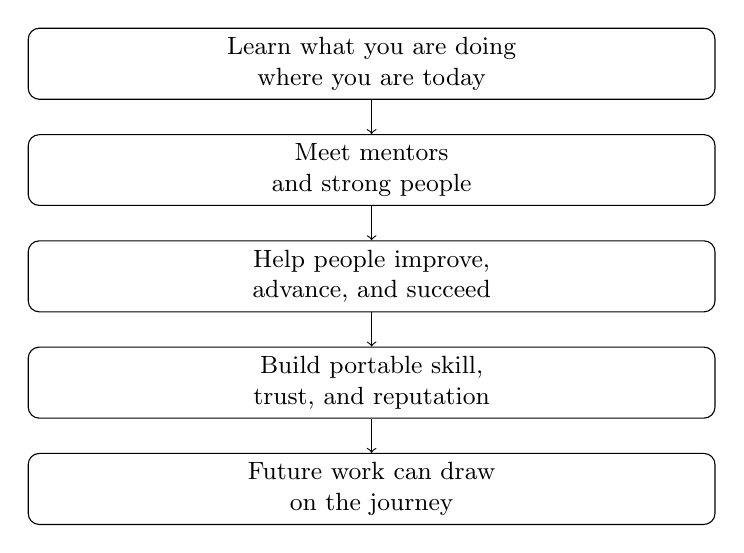
\begin{tikzpicture}[x=1cm,y=1cm,every node/.style={font=\small}]
\node[draw,rectangle,rounded corners,align=center,text width=.70\linewidth] (a) at (0,0) {Learn what you are doing\\where you are today};
\node[draw,rectangle,rounded corners,align=center,text width=.70\linewidth] (b) at (0,-1.35) {Meet mentors\\and strong people};
\node[draw,rectangle,rounded corners,align=center,text width=.70\linewidth] (c) at (0,-2.70) {Help people improve,\\advance, and succeed};
\node[draw,rectangle,rounded corners,align=center,text width=.70\linewidth] (d) at (0,-4.05) {Build portable skill,\\trust, and reputation};
\node[draw,rectangle,rounded corners,align=center,text width=.70\linewidth] (e) at (0,-5.40) {Future work can draw\\on the journey};
\draw[->] (a) -- (b);
\draw[->] (b) -- (c);
\draw[->] (c) -- (d);
\draw[->] (d) -- (e);
\end{tikzpicture}
\caption{A compact reconstruction of the interview's sequence: today's work becomes future value through skill, people, and help given.}
\end{figure}

\subsection{Worked Example: Today's Role}

Suppose we are in a present role \(R_t\). The speaker's advice is not to treat that role as a waiting room for the real career. The role is already producing material for the future if we use it correctly.

\begin{enumerate}
\item We learn what the role requires. That gives \(s_t\), a skill that can remain useful beyond the role.
\item We meet people in and around the role. That gives \(p_t\), a relationship with a mentor, peer, colleague, or future collaborator.
\item We help people get better, move up, and succeed. That gives \(h_t\), a record of contribution that can outlast the reporting line.
\item The present stage then updates the portable stock:
\begin{equation}
\mathcal{J}_{t+1}
=
\mathcal{J}_t \cup \{s_t,p_t,h_t\}.
\end{equation}
\end{enumerate}

We do not know the future role in which \(s_t\), \(p_t\), or \(h_t\) will matter. That uncertainty is part of the speaker's point. The usefulness often appears later, after the work has moved on.

\section{Helping People as Career Leverage}

The middle of the answer is not only about receiving help from mentors. The speaker turns the idea outward. We should care about the people we work with, help them get better, help them move up the food chain, and help them be successful even if they eventually change careers outside our role.

That last clause is important. If someone leaves the immediate role, the narrow organization chart no longer explains the value of helping them. The explanation has to be wider: trust, reputation, gratitude, competence, and the network of people who know how we behave when we have a chance to help.

In the bookkeeping language, help given today is not lost when the person leaves the local setting:

\begin{equation}
h_t \in \mathcal{J}_{t+1}
\quad\text{even when the shared role ends.}
\end{equation}

Again, the notation is only a handle. The interview's real claim is practical: helping people can be one of the most durable forms of entrepreneurial leverage because it travels through people, not through titles.

\section{Learn and Enjoy Today}

The answer resolves into a rule: learn what you are doing where you are today, enjoy what you are doing today, and it will come back and help you in the future. This returns us to the book's working title. Enjoying the walk does not mean ignoring ambition. It means treating the present stage as a real site of learning and contribution.

The word "enjoy" should not be reduced to mere pleasure. In this answer, enjoyment is a form of attention. If we are engaged enough to learn the work, notice the people, and help them improve, then the present role becomes more than a temporary stop.

\section{Summary}

The lecture's movement is simple and useful. It begins with a question about authorship, pivots through the book's working title, looks back from an active later-career vantage point, and identifies what lasted: skills, mentors, people, and help given to others. The job and the company are not dismissed, but they are treated as containers rather than final explanations. The practical rule is to learn and enjoy today's work because the journey itself can become future leverage.